\documentclass[a4paper]{article}
    \title{\vspace{-0.7em}COMS31700: Design Verification - Calculator Design; Testbench Design\vspace{-0.7em}}
    \author{Joshua Van Leeuwen - jv15626 - 23305}
\date{}

\usepackage{titlesec}
\usepackage[margin=0.5in]{geometry}
\geometry{top=10mm, bottom=20mm}


\usepackage{titling}
\usepackage{array}
\usepackage{listings}
\usepackage{graphicx}
\usepackage{wrapfig}

\setlength{\droptitle}{-5em}

\begin{document}
\vspace{-10em}
\maketitle

\vspace{-4.1em}
The testbench uses multiple modules that connect together in order to test the
Design Under Verification (DUV). These contain several structures and units to
create a proper testing environment to collect data against the design
specification.

%The test bench uses 4 modules:
%\begin{enumerate}
%    \item calc1\_sn\_env.e
%    \item driver.e
%    \item coverage.e
%    \item instruction.e
%    \item tests.e
%    \item scoreboard.e
%\end{enumerate}

\subsubsection*{calc1\_sn\_env.e}
\vspace{-0.7em}
This is the top level testbench file. This is used to import all other e
language files into the testbench as well as setting up the the program for
testing. This file will also execute the testbench to start testing on the DUV.

\subsubsection*{instruction.e}
\vspace{-0.7em}
Describes the structures used for testing the DUV. Here the structures are also
extended to be used as the checkers for the structure.

\subsubsection*{driver.e}
\vspace{-0.7em}
File used to drive test data onto the DUV and as well as capture results.  This
is done by executing 4 different test stages - serial, 2 operations in
parallel, 4 in parallel and then testing for priority.  The driver will loop
through each set of instructions and then drive and check the results of that
test. This file also houses the ports to the DUV as well and setting the reset.

\subsubsection*{tests.e}
\vspace{-0.7em}
Here the constraints of the structures are applied for testing. Data input is
constrained to fit in the 32 bit number range with probability to certain
ranges of values. This is in order to ensure that edge and corner case values
are tested for when the test data is being randomly generated. The number of
tests for each test type is also set here. Invalid commands are not to be
tested for for parallel tests since these have already been tested for serially
and would not produce results of interest.

\subsubsection*{coverage.e}
\vspace{-0.7em}
Contains coverage group definitions detailed in the coverage report.

\subsubsection*{scoreboard.e}
\vspace{-0.7em}
Here the scoreboard of the testbench is defined. It is used to test the
priority of the DUV through use of a scoreboard. The scoreboard is implemented
as being a queue which receives sets of ports that are to be expected to be
returned. During the driving of the testbench, if data has been output from the
DUV from a port that is not in the set of ports at the head of the queue then
this means a priority error has occurred; the port has returned before the
previous wave of operations have completed.

\subsubsection*{Testbench Execution Flow}
\vspace{-0.7em}
Shown in Figure 1 is the execution flow of the various modules in the
testbench. Firstly the next set of instructions to be driven are given
to the driver. Here the driver will share or update the relevant structures of
input data to the corresponding modules that are currently enabled. Once
shared, the driver will drive this data onto the DUV. A response collector is
listening to the output of the DUV which will again be used to update or share
this data with the relevant enabled modules to capture the results of the
tests. Once checkers and coverage has been collected from this test, the next
test is ready to be executed from the stimulus generator.
\vspace{-10em}

\begin{figure}
    \centering
    \caption{Execution Flow}
    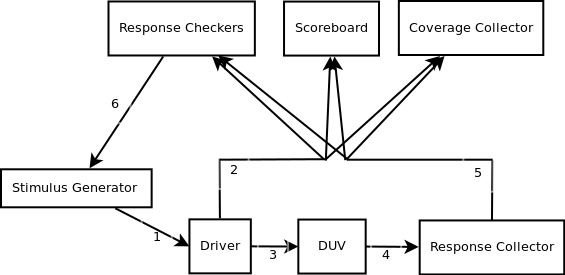
\includegraphics[width=0.7\textwidth]{TestbenchFlow.png}
\end{figure}

\end{document}
